\documentclass{ctexart}
\usepackage{tikz}
\usepackage{circuitikz}
\usepackage{graphicx}

\usepackage[margin=2.5cm]{geometry}
\usetikzlibrary{patterns}

\usepackage{tkz-base,tkz-euclide}

\begin{document}
    \begin{figure}[htp]
        \centering
        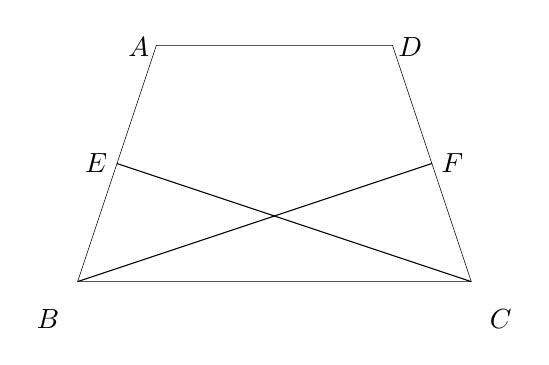
\begin{tikzpicture}
            
            \tkzDefPoints{-2.5/0/B,2.5/0/C,-1.5/3/A,1.5/3/D,0/1.5/O}
            \tkzDefMidPoint(A,B)    \tkzGetPoint{E}
            \tkzDefMidPoint(C,D)    \tkzGetPoint{F}

            \tkzDrawPolygon(A,B,C,D)
            \draw(B) -- (F) node[right]{$F$};
            \draw(C) -- (E) node[left]{$E$};
            \tkzAutoLabelPoints[center=O](A,B,C,D)
        \end{tikzpicture}
        \caption{euclide}
    \end{figure}
\end{document}